\cleardoublepage
\chapter[Koopmans functionals for periodic systems]{Koopmans functionals\break for periodic systems\label{ch:koopmans-periodic}}
In the previous chapter we described the general framework of Koopmans functionals, without focusing on the specific issues that arise when passing from finite to extended systems. Here, we address the issues that are particularly relevant when dealing with infinitely periodic systems, where the need for a localized set of orbitals brings about the apparent breaking of the translation symmetries of the system. The chapter is organized as follows: in Sec.~\ref{sec:localization}, we bring up the importance of having localized sets of variational orbitals in Koopmans functionals and Wannier functions are introduced; in Sec.~\ref{sec:bloch-theorem-section}, we discuss the validity of Bloch's theorem in the framework of ODD functionals, which represents one of the main results of this thesis; finally, Sec.~\ref{sec:koopmans-pbc} is devoted to the formulation of Koopmans functionals in periodic boundary conditions. As usual, we close with a small section that summarizes the content of the chapter.

Part of the content of this chapter has been published in Refs.~\cite{de_gennaro_blochs_2022} and \cite{colonna_koopmans_2022}.

\clearpage
\section{The importance of localization\label{sec:localization}}
Two important aspects underlie the forthcoming discussion about the localization in Koopmans functionals: (i) the discussion at the end of Sec.~\ref{sec:deriv-dis}, and (ii) the nature of the KI correction [see Eq.~\eqref{eq:ki-correction}]. The effects of the orbitals localization on the derivative discontinuity and on the PWL were already touched upon, whereas the impact that such effects can have in infinitely periodic systems, and how this affects Koopmans corrections is the topic of this section.

As usual, we start from standard DFT. It is known that local and semi-local DFAs tend to spread the orbitals as much as possible over the whole system's extension. This is a consequence of the self-interaction error or, equivalently, the deviation from the PWL that affects such approximations, to the point that it has been suggested by Mori-S\'{a}nchez \emph{et al.} to interpret the failures of local functionals in terms of a \emph{delocalization error} \cite{mori-sanchez_localization_2008}. The orbitals delocalization modifies the way the energy deviates from the exact PWL behavior\footnote{Once more, we remark that a correct PWL consists of two equally important features: (i) the linear trend at fractional occupations, and (ii) the correct estimation of the energies on either side of each linear segment, namely the energies at integer numbers of electrons. The fulfillment of the first requirement only, brings to a curve which is, indeed, piecewise-linear, but without the correct slope of the linear segments; in this sense, we consider such a curve to be deviating from the (exact) PWL behavior.}: for finite systems -- the limited extension of the system does not let the orbitals to delocalize too much -- the energy profile is the one showed in the red curve of Fig.~\ref{fig:deviation-pwl}, where the energies at integer points are quite correct, while at fractional occupations we observe a mistaken non-linear convex trend; by increasing the size of the system, the orbitals delocalization increases and the non-linear trend progressively turns into a linear one, while the relative position of the energies at integer numbers of electrons decreases. Such behavior is a natural consequence of the convexity of approximated energy functionals: if we consider a periodic system made of $M$ repetitions of the unit cell, each of which contains $N$ electrons, and we imagine to add a fraction $\delta$ of an electron, Eq.~\eqref{eq:convexity} shows that local functionals will split the electron -- equally, in order to preserve the translation symmetry of the system -- among the different unit cells. The total ground-state energy of the system then reads as \cite{mori-sanchez_localization_2008}
%
\begin{equation}
    \begin{split}
    E^{\rm DFA}(NM + \delta) &= M E^{\rm DFA}\left( N + \frac{\delta}{M} \right) \\
    &= ME^{\rm DFA}(N) + \delta \left. \frac{dE^{\rm DFA}}{dN} \right|_{N+\delta} + \mathcal{O} \left( \frac{\delta^2}{M} \right) .
    \end{split}
    \label{eq:pwl-convex-to-linear}
\end{equation}
%
When approaching the thermodynamic limit ($M\longrightarrow \infty$), the dependence of the energy on $\delta$ becomes more and more linear; moreover, thanks to Janak's theorem
\footnote{The \emph{aufbau} principle tells us that the change in the ground-state energy due to a variation in the number of particles, is equivalent to the one coming from a variation in the occupation of the HO orbital; the Janak's theorem for the HO orbital can then be rewritten as a derivative with respect to the total number of particles:
\begin{equation*}
    \frac{dE}{dN} = \frac{dE}{df_{\rm HO}} = \varepsilon_{\rm HO} .
\end{equation*}
}, 
Eq.~\eqref{eq:pwl-convex-to-linear} shows that the derivative of the energy equals the KS highest-occupied eigenvalue, which strongly underestimates the IP of the system. To summarize, when dealing with infinitely extended systems, the energy of local and semi-local density-functionals shows a linear trend that, at a first sight, might resemble the exact PWL behavior; however, it turns out that, differently from what happens in small finite systems where the orbitals remain localized and $\Delta$SCF-like calculations provide an accurate prediction of ionization energies, here the separation between energies at integer points is strongly underestimated, meaning that not only energy derivatives, but also total energy differences (where an electron was removed from, or added to, a delocalized KS orbital), miss completely the ionization energies of the system.

\begin{figure}
    \centering
    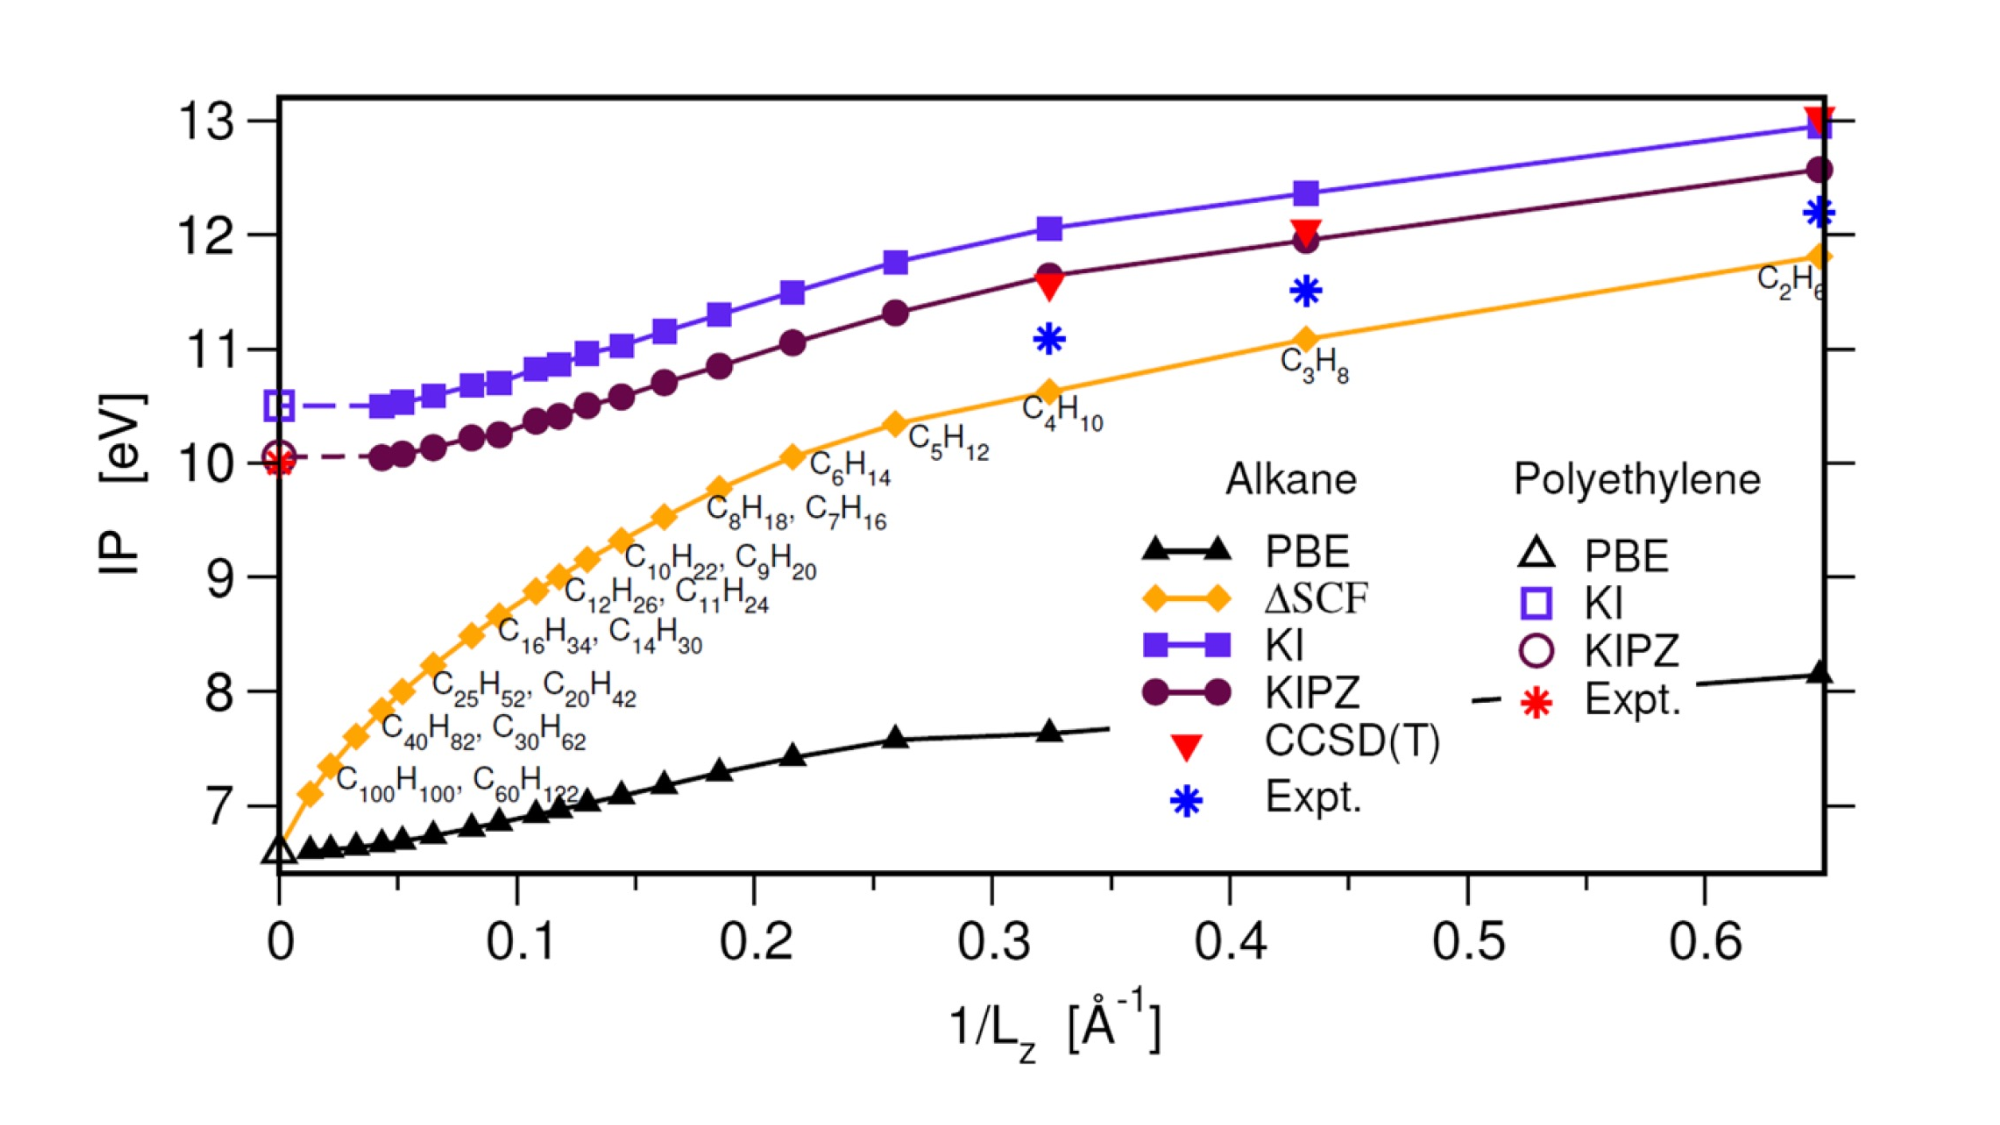
\includegraphics[width=0.80\linewidth]{IP-alkane-chain.pdf}
    \caption[PBE, KI, and KIPZ IPs for the alkane chain.]{A study taken from Ref.~\cite{nguyen_koopmans-compliant_2018}, where the authors compared the performance of PBE, KI, and KIPZ for the calculation of the IP of the alkane chain, $C_n H_{2n}$, at different lenghts, and of polyethylene (infinite limit). The KI and KIPZ IPs are taken as the negative of the HO eigenvalue, while for PBE both $\varepsilon_{\rm HO}$ and the $\Delta$SCF value were considered. At the PBE level, while the opposite of $\varepsilon_{\rm HO}$ strongly underestimates the IP at any lenghts, the $\Delta$SCF value provides accurate predictions at small lenghts and, because of the orbital delocalization, it gets progressively worse when the size of the system increases. We remark that, at the thermodynamic limit, the $\Delta$SCF value recovers the negative of the KS HO eigenvalue. On the other hand, both the Koopmans flavors perfectly agree with coupled-cluster and experimental results (red triangles and star), even at the infinite limit, where the orbitals are represented by (maximally localized) Wannier functions.}
    \label{fig:ip-alkane-chain}
\end{figure}

The failure of local and semi-local DFAs to describe delocalized states becomes crucial when Koopmans corrections are introduced. As we mentioned repeatedly, the KI correction linearizes the energy of the base functional at fractional occupations, and it retains it at integer points. Therefore, for a functional that is already linear, the $\Pi_i^{\rm KI}$ terms of Eq.~\eqref{eq:pi-term-general}, or Eq.~\eqref{eq:ki-correction}, are identically zero. In order to have effective Koopmans corrections in extended systems, it is necessary to switch to a localized representation of the electronic states, where the energy does not vary linearly with respect to a change in the orbital occupations. Rather than considering the Bloch-like KS states, Koopmans functionals resort to sets of localized orbitals -- e.g., Wannier functions -- where the constrained $\Delta$SCF energy differences related to variations in the filling of such orbitals yield, presumably, good results (as shown in Fig.~\ref{fig:ip-alkane-chain}).

The advantage of using localized orbitals has driven many DFT-based methods that aimed to describe excited-state properties of periodic systems -- some of those introduce corrections that closely resemble the KI functional. To mention a few we find: the transition-state method proposed by Anisimov and collaborators, which generalizes Slater's $1/2$-method by improving the definition of the ionization energies -- rather than taking the values of the energy curvature, $\partial \varepsilon_i / \partial f_i$, at half occupation, these are computed self-consistently via constrained DFT calculations -- and by replacing the KS Bloch states, for which the applied corrections vanish in extended systems, with Wannier functions \cite{anisimov_transition_2005,anisimov_orbital_2007}; the range-separated dielectric-dependent hybrid functionals developed by Wing \emph{et al.}, where the optimal value of the range-separation parameter is determined by imposing the Koopmans condition on the Wannier functions, rather than on the delocalized KS states \cite{wing_band_2021}; the Wannier-Koopmans method developed in the group of L.-W. Wang, which augments the LDA Hamiltonian with Wannier-based $\Delta$SCF-like terms \cite{ma_using_2016,ma_energy_2016,weng_wannier_2017,weng_wannier_2018,li_wannier-koopmans_2018,weng_wannierkoopmans_2020}; similar corrections are used also in the localized orbital scaling correction (LOSC) scheme developed by W. Yang and collaborators, who make use of Wannier-like \emph{orbitalets} (orbitals obtained by finding the optimal compromise between the localization in space and in energy) \cite{li_localized_2018,mei_libsc_2021,mahler_wannier_2022}.

Also in PZ-SIC functionals, the orbitals localization plays a fundamental role: the density of a delocalized orbital is locally very small, and the correspondent self-Hxc energy tends rapidly to zero. This explains why PZ corrections vanish in the limit of infinitely extended systems, and provides further evidence for the disappearance of Koopmans corrections:
%
\begin{equation}
    \begin{split}
    \Pi_i^{\rm uKI} &= E^{\rm DFT}[\rho - \rho_i] - E^{\rm DFT}[\rho] + f_i \left( E^{\rm DFT}[\rho - \rho_i + n_i] - E^{\rm DFT}[\rho - \rho_i] \right) \\
    &\approx E^{\rm DFT}[\rho] - E^{\rm DFT}[\rho] + f_i \left( E^{\rm DFT}[\rho] - E^{\rm DFT}[\rho] \right) = 0 .
    \end{split}
    \label{eq:vanishing-ki-correction}
\end{equation}
%
The minimization of the PZ energy naturally brings to a set of localized orbitals\footnote{We point out that, in order to localize the orbitals, SIC schemes often require the initial guess to be already localized, whereas starting from delocalized orbitals might bring to local minima where the orbitals are still delocalized \cite{korzdorfer_relation_2011}.} -- closely resembling Foster-Boys orbitals \cite{boys_construction_1960,foster_canonical_1960} in finite systems, and maximally localized Wannier functions \cite{marzari_maximally_1997,marzari_maximally_2012} in extended periodic systems \cite{nguyen_koopmans-compliant_2018} -- for which the magnitude of $E_{\rm Hxc}[\rho_i]$ increases, and the system reaches a more energetically favorable configuration (the self-Hxc terms are preceded by the negative sign, thus the energy is minimized by maximizing such terms). In this sense, the Pederson condition, which provides the energy minima within a particular subspace, is also interpreted as a \emph{localization condition}. Given the equivalence between Koopmans' and PZ's gradients -- we remind that KIPZ is the KI correction applied to a screened PZ functional, while KI can be seen as a KIPZ functional with a vanishigly small PZ term -- the minimization of Koopmans functionals benefits from the same ``natural'' predisposition to localize orbitals and, ultimately, allows to have effective Koopmans corrections also in extended systems.

\subsection{Wannier functions\label{sec:wannier-functions}}
When dealing with periodic systems, the most natural choice for a set of localized orbitals is represented by Wannier functions (WFs) \cite{wannier_structure_1937}. The reason is that WFs possess important properties that carry all the information about the translation symmetries of the system. Moreover, WFs are strictly connected to Bloch functions (BFs), as they reciprocally play the role of Fourier transforms of the other, which makes them the dual representation of Bloch states\footnote{To be exact, there is an arbitrary component in the definition which prevents WFs from having a one-to-one correspondence with BFs; this concept will be further discussed in the section.}.

Given the set $\{ \psink \}$ of BFs, where $\bk$ are the crystal vectors living within the (first) Brillouin zone (BZ) of the system, the most general definition for a Wannier function $\wnR$, corresponding to the Bravais lattice (BL) vector $\bR$ and with band index $n$, is
%
\begin{equation}
    \ket{\wnR} = \frac{1}{\Omega} \int_{\Omega} d\bk \ e^{-i\bk \cdot \bR} \sum_m U^{(\bk)}_{mn} \ket{\psi_{m\bk}} ,
    \label{eq:wannier-function}
\end{equation}
%
where $\Omega = 8\pi^3 / V$ is the volume of the BZ. The $U^{(\bk)}_{mn}$ are unitary matrices mixing BFs with the same crystal momentum, and their presence is a consequence of the gauge freedom that characterizes the definition of WFs. In fact, for a given set of BFs, an infinite set of WFs -- one for each $U^{(\bk)}$ -- can be defined. Such arbitrariness needs to be resolved in order to arrive to an unambiguous definition of WFs: the infamous Marzari-Vanderbilt localization criterion \cite{marzari_maximally_1997}, provides a solution to this problem by means of a minimization procedure, and it will be further discussed at the end of the section. As a consequence of the orthogonality of the Bloch states, also WFs turn out to be orthogonal, i.e.
%
\begin{equation}
    \braket{\wnR | w_{m\bR'}} = \delta_{nm} \delta_{\bR \bR'} .
    \label{eq:orthogonality-wannier}
\end{equation}
%
It follows from Eq.~\eqref{eq:wannier-function}, that WFs fulfill the translation property
%
\begin{equation}
    \wnR(\br + \bR') = w_{n\bR - \bR'}(\br) ,
    \label{eq:trans-prop-wannier}
\end{equation}
%
for any pair of BL vectors $(\bR,\bR')$, where $\wnR(\br) = \braket{\br|\wnR}$ is the real-space projection of the Wannier function. In order to highlight the importance of property \eqref{eq:trans-prop-wannier}, let us consider, for simplicity, a simple 1-band case (the band index is dropped), and show that an orthonormal set of one-particle wave functions satisfying such property, can be expressed in terms of the BFs as in Eq.~\eqref{eq:wannier-function}. To prove it, let us assume that the set of orbitals $\{ \wR \}$ is orthonormal and satisfies Eq.~\eqref{eq:trans-prop-wannier}; since the Bloch states represent a basis for the Hilbert space, we can express $\wR$ as a linear combination of BFs,
%
\begin{equation}
    \wR(\br) = \frac{1}{\Omega} \int_{\Omega} d\bk \ C(\bR,\bk) \psik(\br) .
    \label{eq:wannier-bloch-linear-combination}
\end{equation}
%
By imposing Eq.~\eqref{eq:trans-prop-wannier}, we obtain the following condition for the coefficients:
%
\begin{equation}
    C(\bR + \bR', \bk) = C(\bR, \bk) e^{-i\bk \cdot \bR'} ,
    \label{eq:crk-coefficents-trans-prop}
\end{equation}
%
valid for any pair of BL vectors $(\bR,\bR')$, and for any $\bk$ in the BZ. By choosing $\bR=0$, we can factor out the $\bR$-dependence of the coefficients
%
\begin{equation}
    C(\bR',\bk) = C(\bk) e^{-i\bk \cdot \bR'} ,
    \label{eq:crk-coefficients-factor-out}
\end{equation}
%
and, finally, the orthonormality of $\{ \wR \}$ forces the coefficients to be unitary, i.e. $|C(\bk)|^2=1$, from which we conclude that
\begin{equation}
    C(\bk) = e^{i\varphi(\bk)} ,
\end{equation}
%
for some function $\varphi(\bk)$, which represents the aforemonetioned gauge freedom of WFs -- for 1-band systems the matrix $U^{(\bk)}$ reduces to $e^{i\varphi(\bk)}$.

To conlcude this part, we point out that thanks to property \eqref{eq:trans-prop-wannier}, Wannier functions contain all the information about the translation symmetries of the system, as much as BFs do. Essentially, while for the latter this information is owned by each function independently, in the case of Wannier functions is only by considering the whole set of functions that one can gather the information about the translation symmetries of the system.

\subsubsection*{Maximally localized Wannier functions}
As mentioned earlier, the definition of Wannier functions is not univocal, as for a given set of BFs, WFs are defined up to a unitary transformation (block-diagonal, over $\bk$). The Marzari-Vanderbilt localization criterion is one of the most successful methods to solve such ambiguity, since it brings to a set of \emph{maximally localized Wannier functions} (MLWFs) \cite{marzari_maximally_1997}, which have proved to be extremely useful to interpolate the electronic bands, and to compute many physical properties \cite{marzari_maximally_2012} -- including the electric polarization, the orbital magnetization, and the electron-phonon coupling -- otherwise difficult to handle with a delocalized set of orbitals.

The method aims to find the unitary transformation $U^{(\bk)}$ which minimizes the variance of the position operator:
%
\begin{equation}
    \min_{\{ U^{(\bk)} \}} \ \sum_n \left[ \langle r^2 \rangle_{w_n} - \langle \br \rangle_{w_n}^2 \right] ,
    \label{eq:wannier-spread-functional}
\end{equation}
%
where $\langle \cdot \rangle_{w_n}$ indicates the expectation value over $w_{n{\bm 0}}$ -- given the translation property \eqref{eq:trans-prop-wannier}, it is enough to evaluate the spread functional of Eq.~\eqref{eq:wannier-spread-functional} over a single lattice vector, e.g., $\bR = \bm 0$. MLWFs are then an extension of Foster-Boys molecular orbitals (defined by the same localization procedure) \cite{boys_construction_1960,foster_canonical_1960} to periodic systems, and represent a very good guess for the PZ and Koopmans variational orbitals. Indeed, as discussed before, such variational orbitals result from the maximization of the Hxc self-interaction terms which, for local or semi-local approximations, are usually dominated by the self-Hartree energy. The maximization of the Hartree self-interaction represents an alternative localization scheme yielding orbitals that are very similar to MLWFs \cite{marzari_maximally_2012}. Ultimately, all these observations justify the use of MLWFs either as a non-self-consistent guess for the variational orbitals, or as a starting point for the minimization, when performing calculations of Koopmans functionals in periodic systems.

To end this section, we point out that MLWFs are only one of the infinite choices for a set of localized orbitals, even in periodic systems. The previous argument highlights the importance of having a set of (maximally) localized orbitals but, in principle, does not impose any particular constraint, such as the translation property \eqref{eq:trans-prop-wannier}. However, Wannier-like orbitals are compliant the translation symmetries of the system and, as we shall see in the next section, they play a fundamental role in the fulfillment of Bloch's theorem in ODD functionals.

\section{Bloch's theorem in ODD functionals\label{sec:bloch-theorem-section}}
The need for a set of localized orbitals brings about a fundamental problem in periodic systems: a localized orbital density does not have the periodicity of the primitive cell, which means that the potential built on such density -- such as any ODD potential present in the Koopmans Hamiltonian -- breaks the translation symmetry of the system. The periodicity of the effective potential is required by Bloch's theorem, whereas the lack of this feature prevents from describing the one-particle spectrum via a band structure picture (which represents an actual physical observable that can be gauged via, e.g., the ARPES experiment). In this section -- representing the central result of this thesis -- we show that rather than focusing on the individual non-periodic ODD potentials, the object to consider is the Koopmans Hamiltonian (or the Koopmans potential) introduced in Sec.~\ref{sec:koopmans-hamiltonian}; as long as the localized orbitals keep a Wannier-like form\footnote{With Wannier-like form, we mean that the orbitals fulfill the translation property \eqref{eq:trans-prop-wannier}, and therefore are in effect Wannier functions.}, the Koopmans Hamiltonian is periodic and fulfills Bloch's theorem.

We start introducing Bloch's theorem in a general framework (Sec.~\ref{sec:bloch-theorem}), and then we discuss its validity in the case of standard density-functionals (Sec.~\ref{sec:bloch-th-dft}), and of orbital-density-dependent approaches (Sec.~\ref{sec:bloch-th-odd}).

\subsection{Bloch's theorem\label{sec:bloch-theorem}}
For any approach relying on the independent-particle approximation, Bloch's theorem represents a fundamental result which reduces enormously the complexity of the electronic Hamiltonian of a periodic system. As a consequence of Bloch’s theorem, and more generally of group theory, the irreducible representations -- labeled by the crystal vectors $\bk$ -- of the system's translation group allow for a block-diagonal representation of the Hamiltonian, which brings to a band structure description of the energy spectrum. The only requirement of Bloch's theorem then, is the commutativity of the Hamiltonian with a (closed) set of symmetry operations, which, in a crystal, correspond to the translation group of the underlying BL: $\{ \tR \}$.

In a local mean-field approach, the commutativity of the Hamiltonian with the set of translation operators, reduces to the periodicity of the effective local potential, $v_{\rm eff}(\br)$, over the BL vectors $\bR$. The Hamiltonian can then be co-diagonalized with the set of operators $\{ \tR \}$, and the resulting eigenvectors take the form of \emph{Bloch functions}
%
\begin{equation}
    \psink(\br) = e^{i\bk \cdot \br} u_{n\bk}(\br)
    \qquad \text{with} \qquad
    u_{n\bk}(\br+\bR) = u_{n\bk}(\br) ,
    \label{eq:bloch-functions}
\end{equation}
%
where the BFs are eigenvectors of the translation operators with eigenvalue $e^{i\bk \cdot \br}$. On the basis of BFs, the Hamiltonian takes a block-diagonal form where each block corresponds to a specific $\bk$-vector and solves the eigenvalue problem
%
\begin{equation}
    H_{\bk}(\br) u_{n\bk}(\br) = \varepsilon_{n\bk} u_{n\bk}(\br)
    \qquad \text{with} \qquad
    H_{\bk}(\br) = - \frac{(\nabla + i\bk)^2}{2} + v_{\rm eff}(\br) .
    \label{eq:k-block-crystal-ham}
\end{equation}
%
The eigenvalues $\varepsilon_{n\bk}$ of the Hamiltonian acquire a new quantum number $\bk$, which labels the irreps of the translation group and gives rise to the band structure description of the spectrum.

\subsection{Validity in standard DFT\label{sec:bloch-th-dft}}
For local and semi-local approximations of the xc functional, the KS potential is made of a term that does not depend (explicitly) on the total density -- the external potential, $v(\br)$ -- and a part whose spatial dependence is totally determined by $\rho(\br)$ -- namely the Hartree and xc potentials, $v_{\rm Hxc}[\rho](\br)$. In a crystalline material, $v(\br)$ is given by the electrostatic potential of the nuclei which has, by construction, the periodicity of the BL; on the other hand, the Hxc potential is periodic only if the density is. If we exclude exotic ground states -- like those with charge-density waves, where the periodicity of the density is not commensurate with that of the lattice -- the density $\rho(\br)$ resulting from the energy minimization is periodic, which makes the Hxc -- and, thus, the KS effective potential -- periodic and compliant with Bloch's theorem.

When performing standard primitive cell (PC) calculations\footnote{The primitive cell is the smallest possible unit cell; when speaking of primitive cell calculations, we implicitly assume a sufficient sampling of the BZ that allows to model the thermodynamic bulk limit of the material.}, the periodicity of the density is assumed \emph{a priori} and the KS states are defined as BFs: Bloch's theorem is trivially satisfied, and the band structure results effortlessly from the calculation. The same system can be simulated without imposing the translation symmetry, via a supercell (SC) calculation\footnote{In this thesis, for supercell calculations, we always refer to calculations over unit cells with a bigger periodicity of the PC, where the sampling of the BZ consists of a single point ($\Gamma$-point-only sampling); the defined supercell demarcates the whole (simulated) system's volume, and usually demands for a higher computational cost with respect to PC calculations (the latter indeed takes full advantage of Bloch's theorem).}: in this case, unless the system lowers its energy by breaking the translation symmetry, the periodicity of the density emerges naturally during the energy minimization, and Bloch's theorem still holds. However, we point out that in this case, although a band structure description does exist, the KS orbitals are not constrained to be BFs and an unfolding method (like the one discussed in Sec.~\ref{sec:unfolding-method}) that reconstructs the connection between the energy eigenvalues and the points of the PC's BZ, is required.

\subsection{Validity in ODD functionals\label{sec:bloch-th-odd}}
At odds with DFT, where the total density is the only quantity entering the Hamiltonian, Koopmans functionals (and their Hamiltonians) depend on the set of variational orbital densities, and therefore the periodicity (over the primitive cell) of the total density alone is not sufficient to obtain a periodic potential. In this case a more stringent condition is needed, and in the following we show that this extra condition is given by the Wannier-like character of the variational orbitals. If the variational orbitals satisfy Eq.~\eqref{eq:trans-prop-wannier}, the Koopmans potential \eqref{eq:koopmans-potential} turns out to have the periodicity of the PC and, therefore, the Koopmans Hamiltonian \eqref{eq:koopmans-hamiltonian} fulfills the hypothesis of Bloch's theorem \cite{de_gennaro_blochs_2022}.

Below, we show the compliance of the Koopmans Hamiltonian with Bloch's theorem, where the only assumption is the Wannier nature of the variational orbitals (which actually implies the periodicity of the total density). Since the Koopmans potential is a combination of several PZ-like terms, for simplicity here we give the mathematical proof for the PZ potential and for a 1-band system, while we refer to Appendix~\ref{app:periodic-ki-kipz} for the full derivation for the KI and KIPZ Hamiltonians. Definitions \eqref{eq:koopmans-hamiltonian} and \eqref{eq:koopmans-hamiltonian-equivalent-definition} are readily extended to the PZ potential, which on the set of variational WFs $\{ \wR \}$ reads as
%
\begin{subequations}
    \begin{equation}
        \vpz = \sum_{\bR} \vpz_{\bR} \ket{\wR} \bra{\wR}
        \label{eq:pz-potential-def-1}
    \end{equation}
    \begin{equation}
        \vpz = \sum_{\bR, \bR'} v^{\rm PZ}_{\bR \bR'} \ket{\wR} \bra{\wRp}
        \label{eq:pz-potential-def-2}
    \end{equation}
    \label{eq:pz-potential}
\end{subequations}
%
where $\rho_{\bR}(\br) = f_{\bR} |w_{\bR}(\br)|^2$, $\vpz_{\bR} = - \hat{v}_{\rm Hxc}[\rho_{\bR}]$, and $v^{\rm PZ}_{\bR \bR'} = \braket{\wR | \vpz_{\bR'} | \wRp}$. To further show the equivalence between the two definitions, we will prove that in both cases the PZ potential commutes with all the translation operators:
%
\begin{equation}
    \left[ \vpz, \tR \right] = 0 \qquad \qquad \forall \bR \in {\rm BL} .
    \label{eq:commutativity-pz-potential}
\end{equation}
%
In the following steps, we make use of the properties of the translation operators, whose action over any function $\psi(\br)$ is given by $\tR: \psi(\br) \longrightarrow \psi(\br + \bR)$. In Dirac's notation, the action of the translation operators is defined on the positional kets $\ket{\br}$ as
%
\begin{equation}
    \tR \ket{\br} = \ket{\br - \bR} ,
    \label{eq:action-trans-operator}
\end{equation}
%
which is, indeed, consistent with the previous definition:
%
\begin{equation}
    \begin{split}
        \tR \psi(\br) &= \braket{\br|\tR|\psi} \\
        &= \int d\br' \ \braket{\br|\tR|\br'} \braket{\br'|\psi} \\
        &= \int d\br' \ \braket{\br|\br'-\bR} \psi(\br') \\
        &= \psi(\br + \bR) .
    \end{split}
\end{equation}

\subsubsection*{Case A: $\vpz = \sum_{\bR} \vpz_{\bR} \ket{\wR} \bra{\wR}$}
As shown in Appendix~\ref{app:periodic-ki-kipz}, the occupation number of the Wannier functions are independent from the lattice vector, i.e. $f_{\bR} = f_{\bm 0}$. By definition, the Wannier orbital densities $\rho_{\bR}(\br) = f_{\bm 0} |w_{\bR}(\br)|^2$ fulfill the same translation property \eqref{eq:trans-prop-wannier} as $w_{\bR}(\br)$:
%
\begin{equation}
    \rho_{\bR}(\br + \bR') = \rho_{\bR - \bR'}(\br) .
    \label{eq:trans-prop-wannier-orb-dens}
\end{equation}
%
The crucial step is to show that also the ODD potentials $\hat{v}_{\rm Hxc}[\rho_{\bR}]$ satisfy the same property. Let us consider the self-Hartree potential first:
%
\begin{equation}
    \begin{split}
        v_{\rm H}([\rho_{\bR}],\br + \bR') & = \int_V d\br' \frac{\rho_{\bR}(\br')}{|\br + \bR' - \br'|} \\ 
        & = \int_V d\br' \frac{\rho_{\bR}(\br' + \bR')}{|\br - \br'|} \\
        & = \int_V d\br' \frac{\rho_{\bR - \bR'}(\br')}{|\br - \br'|} \\
        & = v_{\rm H}([\rho_{\bR - \bR'}],\br) ,
    \end{split}
    \label{eq:trans-prop-hartree-pot}
\end{equation}
%
where $V$ is the supercell volume, and we made use of Eq.~\eqref{eq:trans-prop-wannier-orb-dens}. For the self-xc potentials $\hat{v}_{\rm xc}[\rho_{\bR}]$ the situation is even simpler; at LDA and GGA levels, the xc functional is generally given by Eq.~\eqref{eq:gga-xc}, hence the xc potential $v^{\rm xc}([\rho_{\bR}],\br) = \frac{df}{d\rho_{\bR}}(\rho_{\bR}(\br), \nabla\rho_{\bR}(\br))$ inherits the full $\br$-dependence from the density. It is straightforward then, to show that $v_{\rm xc}([\rho_{\bR}],\br + \bR') = v_{\rm xc}([\rho_{\bR - \bR'}],\br)$, which finally yields the following property for the PZ ODD potential terms
%
\begin{equation}
    v^{\rm PZ}_{\bR}(\br + \bR') = v^{\rm PZ}_{\bR - \bR'}(\br) ;
    \label{eq:trans-prop-pz-pot}
\end{equation}
%
Eq.~\eqref{eq:trans-prop-pz-pot} is sufficient to prove the final argument:
%
\begin{equation}
    \begin{split}
        \tR \vpz \ket{\psi} &= \sum_{\bR'} \tR \vpz_{\bR'} \ket{\wRp} \braket{\wRp|\psi} \\
        &= \sum_{\bR'} \int d\br \ \tR \ket{\br} \braket{\br|\vpz_{\bR'}|\wRp} \int d\br' \ \braket{\wRp|\br'} \braket{\br'|\psi} \\
        &= \sum_{\bR'} \int d\br \ \ket{\br - \bR} v^{\rm PZ}_{\bR'}(\br) \wRp(\br) \int d\br' \ \wRp^*(\br') \psi(\br') \\
        &= \sum_{\bR'} \int d\br \ \ket{\br} v^{\rm PZ}_{\bR'}(\br + \bR) \wRp(\br + \bR) \int d\br' \ w_{\bR' - \bR}^*(\br') \psi(\br' + \bR) \\
        &= \sum_{\bR'} \int d\br \ \ket{\br} v^{\rm PZ}_{\bR' - \bR}(\br) w_{\bR' - \bR}(\br) \int d\br' \ \braket{w_{\bR' - \bR}|\br'} \braket{\br'|\tR|\psi} \\
        &= \int d\br \ \ket{\br} \bra{\br} \left( \sum_{\bR'} \vpz_{\bR' - \bR} \ket{w_{\bR' - \bR}} \bra{w_{\bR' - \bR}} \right) \tR \ket{\psi} \qquad (\bR' - \bR \longrightarrow \bR') \\
        &= \vpz \tR \ket{\psi} ,
    \end{split}
    \label{eq:demonstration-commutativity}
\end{equation}
%
where we used the fact that $\{ \bR \}$ is a closed set. The result above applies to any state $\ket{\psi}$ and, therefore, proves the validity of Eq.~\eqref{eq:commutativity-pz-potential}.

\subsubsection*{Case B: $\vpz = \sum_{\bR, \bR'} v^{\rm PZ}_{\bR \bR'} \ket{\wR} \bra{\wRp}$}
In this case, the property that allows to prove the commutativity of the PZ potential regards the matrix elements of the PZ potential. From Eq.~\eqref{eq:trans-prop-pz-pot}, it follows that
%
\begin{equation}
    \begin{split}
        v^{\rm PZ}_{\bR+\bR'',\bR'} &= \braket{w_{\bR+\bR''} | \hat{v}^{\rm PZ} | w_{\bR'}} \\
        &= \int d\br\ w^*_{\bR+\bR''}(\br) v^{\rm PZ}_{\bR'}(\br) w_{\bR'}(\br) \\
        &= \int d\br\ w^*_{\bR}(\br) v^{\rm PZ}_{\bR'-\bR''}(\br) w_{\bR'-\bR''}(\br) \\
        &= \braket{w_{\bR} | \hat{v}^{\rm PZ} | w_{\bR'-\bR''}} \\
        &= v^{\rm PZ}_{\bR,\bR'-\bR''} .
    \end{split}
    \label{eq:trans-prop-matrix-element}
\end{equation}
%
This can then be used to prove the commutativity of the PZ potential defined as in Eq.~\eqref{eq:pz-potential-def-2}:
%
\begin{equation}
    \begin{split}
        \tR \vpz \ket{\psi} &= \sum_{\bR',\bR''} v^{\rm PZ}_{\bR' \bR''} \tR \ket{\wRp} \braket{w_{\bR''}|\psi} \\
        &= \sum_{\bR',\bR''} v^{\rm PZ}_{\bR' \bR''} \int d\br \ \ket{\br - \bR} \wRp(\br) \braket{w_{\bR''}|\psi} \\
        &= \sum_{\bR',\bR''} v^{\rm PZ}_{\bR' \bR''} \int d\br \ \ket{\br} w_{\bR'- \bR}(\br) \braket{w_{\bR''}|\psi} \qquad (\bR' - \bR \longrightarrow \bR') \\
        &= \sum_{\bR',\bR''} v^{\rm PZ}_{\bR'+\bR,\bR''} \int d\br \ \ket{\br} \braket{\br|\wRp} \braket{w_{\bR''}|\psi} \\
        &= \sum_{\bR',\bR''} v^{\rm PZ}_{\bR',\bR''-\bR} \ket{\wRp} \braket{w_{\bR''}|\psi} \qquad \qquad \qquad (\bR''-\bR \longrightarrow \bR'') \\
        &= \sum_{\bR',\bR''} v^{\rm PZ}_{\bR',\bR''} \ket{\wRp} \int d\br \ w_{\bR''+\bR}^*(\br) \psi(\br) \\
        &= \sum_{\bR',\bR''} v^{\rm PZ}_{\bR',\bR''} \ket{\wRp} \bra{w_{\bR''}} \int d\br \ \ket{\br-\bR} \psi(\br) \\
        &= \vpz \int d\br \ \tR \ket{\br} \braket{\br|\psi} \\
        &= \vpz \tR \ket{\psi} ,
    \end{split}
\end{equation}
%
where, also here, we used the closure of $\{ \bR \}$, together with the properties of the translation operators.

The extension to the whole PZ Hamiltonian is trivial, since the remainder part is the DFT Hamiltonian which commutes already with all the translation operators. Although the Koopmans Hamiltonian is more complex than the PZ one discussed here, it is made of orbital-density-dependent potentials of the very same nature of the PZ ones, alongside scalar terms -- meaning that they do not depend on $\br$ -- or terms that depend only on the total density $\rho$. The latter are trivially periodic on the primitive cell because of the periodicity of the total density (see Appendix~\ref{app:periodic-ki-kipz} for a detailed derivation). The proof given above thus readily applies also to the Koopmans Hamiltonian \eqref{eq:koopmans-hamiltonian} -- and actually to any PZ-like ODD approach -- which then fulfills the hypotesis of Bloch's theorem, i.e.
%
\begin{equation}
    \left[ \tR, \hat{h}^{\rm KC} \right] = 0 .
    \label{eq:commutativity-koopmans-ham}
\end{equation}
%
It is important to stress that Eq.~\eqref{eq:commutativity-koopmans-ham} proves the existence of a band structure description of the quasiparticle spectrum resulting from the Koopmans Hamiltonian, however, the computation of the self-interaction terms on the localized orbitals still requires to deal with non-periodic orbital densities. The standard approach then requires calculations in a supercell, where the information about the $\bk$-dependence of the eigenenergies is not given explicitly. An unfolding method that allows to reconstruct this information is needed, and in the following chapter we will describe the strategy used in this work

To summarize, we have shown that when the variational orbitals are Wannier functions (i.e.\ they satisfy Eq.~\eqref{eq:trans-prop-wannier}) the potential $\hat{v}^{\rm KC}$ defined in Eq.~\eqref{eq:koopmans-hamiltonian} is periodic over the PC, making the Koopmans Hamiltonian Bloch-compliant. As an aside, the Wannier-like nature of the orbitals and the Bloch-compliance of Koopmans functionals also makes it possible to develop a PC implementation of Koopmans functionals, for direct access to the band structure without the need of supercell calculations and of an unfolding procedure \cite{colonna_koopmans_2022}; a brief overview of this implementation is given in the following section. As we already mentioned above, the assumption of having Wannier-like variational orbitals is justified by the observation that the minimization of Koopmans and PZ functionals in extended systems leads to orbitals with these properties. While this has occurred in all the systems so far considered, it is important to remark that the lack of the Wannier-like character in the variational orbitals would prevent from applying the Bloch's theorem and implies the actual breaking of the translation symmetry of the system. Such situations are presumably as sporadic as when in standard DFT the periodicity of the ground-state density is not commensurate to that of the lattice potential and they should not be confused with special system-dependent gauge invariances that Koopmans functionals might have. Despite the non-unitary invariance of the functionals, there is indeed no guarantee for the uniqueness of the set of variational orbitals and we cannot exclude \emph{a priori} that there might exist some gauges for which the translation symmetry of the lattice is broken.

\section{Koopmans functionals in periodic boundary conditions\label{sec:koopmans-pbc}}

\section{Summary\label{sec:ch4-summary}}

